\documentclass[10pt,a4paper]{article}
% Compiles with pdflatex (+ bibtex) and with Tectonic/XeLaTeX. Sources are ASCII-only.
\usepackage{iftex}
\ifPDFTeX
  \usepackage[utf8]{inputenc}
  \usepackage[T1]{fontenc}
\fi
\usepackage{lmodern}
\usepackage[margin=2cm]{geometry}
% shared packages, notation and generated numbers for the end-evaluation report, slides and appendix
\usepackage{amsmath,amssymb}
\usepackage{booktabs}
\usepackage{graphicx}
\usepackage{siunitx}
\usepackage{xcolor}
\usepackage{adjustbox}
\makeatletter
\providecommand{\input@path}{}
\g@addto@macro\input@path{{.}{docs/}{./docs/}{../docs/}}
\makeatother
\graphicspath{{../figures/nine_crop/}{../figures/four_crop/}{figures/nine_crop/}}
% generated by code/19_endeval_tex.py -- do not edit
\newcommand{\nPairs}{59}
\newcommand{\nCountries}{20}
\newcommand{\nCrops}{9}
\newcommand{\orderEq}{Wheat $>$ Maize $>$ Common bean $>$ Soybean $>$ Rapeseed-mustard $>$ Chickpea $>$ Rice $>$ Lentil $>$ Groundnut}
\newcommand{\topEq}{Wheat}
\newcommand{\secondEq}{Maize}
\newcommand{\lastEq}{Groundnut}
\newcommand{\topEqValue}{0.0563}
\newcommand{\secondEqValue}{0.0297}
\newcommand{\orderPw}{Wheat $>$ Common bean $>$ Chickpea $>$ Rapeseed-mustard $>$ Soybean $>$ Maize $>$ Lentil $>$ Groundnut $>$ Rice}
\newcommand{\topPw}{Wheat}
\newcommand{\secondPw}{Common bean}
\newcommand{\lastPw}{Rice}
\newcommand{\topPwValue}{0.0696}
\newcommand{\secondPwValue}{0.0233}
\newcommand{\topPairA}{wheat--Russia}
\newcommand{\topPairAValue}{0.1315}
\newcommand{\topPairB}{maize--South Africa}
\newcommand{\topPairBValue}{0.1237}
\newcommand{\topPairC}{wheat--USA}
\newcommand{\topPairCValue}{0.0903}
\newcommand{\topPairD}{wheat--India}
\newcommand{\topPairDValue}{0.0676}
\newcommand{\topPairE}{common bean--Brazil}
\newcommand{\topPairEValue}{0.0459}
\newcommand{\topPairF}{common bean--Tanzania}
\newcommand{\topPairFValue}{0.0357}
\newcommand{\refHeatPair}{common bean--India}
\newcommand{\refHeat}{5.046}
\newcommand{\refWaterPair}{chickpea--India}
\newcommand{\refWater}{0.789}
\newcommand{\refImpPair}{rice--Bangladesh}
\newcommand{\refImp}{0.421}
\newcommand{\groupOrder}{Cereals $>$ Pulses $>$ Oilseeds}
\newcommand{\nDivUnits}{21}
\newcommand{\wheatTopZinc}{16}
\newcommand{\wheatTopIron}{15}
\newcommand{\wheatTopProtein}{9}
\newcommand{\wheatTopKcal}{14}
\newcommand{\maizeSAkcal}{22}
\newcommand{\maizeSArainfed}{89}
\newcommand{\maizeSAEwater}{0.46}
\newcommand{\maizeUAEwater}{0.61}
\newcommand{\maizeFoodUSA}{1}
\newcommand{\maizeFoodChina}{3}
\newcommand{\maizeFoodSA}{40}
\newcommand{\futHeatShare}{72}
\newcommand{\futWaterShare}{28}
\newcommand{\nPairsDown}{14}
\newcommand{\nPairsDownWaterOnly}{14}
\newcommand{\futOrderEq}{Wheat $>$ Maize $>$ Common bean $>$ Rapeseed-mustard $>$ Soybean $>$ Chickpea $>$ Rice $>$ Lentil $>$ Groundnut}
\newcommand{\histOrderEq}{Wheat $>$ Maize $>$ Common bean $>$ Soybean $>$ Rapeseed-mustard $>$ Chickpea $>$ Rice $>$ Groundnut $>$ Lentil}
\newcommand{\futOrderPw}{Wheat $>$ Common bean $>$ Chickpea $>$ Rapeseed-mustard $>$ Soybean $>$ Maize $>$ Lentil $>$ Groundnut $>$ Rice}
\newcommand{\nPairsUp}{40}
\newcommand{\nPairsExceedRef}{1}
\newcommand{\meanDTeff}{1.9}
\newcommand{\futTopPair}{wheat--Russia}
\newcommand{\futTopPairChange}{+0.0207}
\newcommand{\climCheckSameSign}{92}
\newcommand{\climCheckRho}{0.96}
\newcommand{\histReproMaxDiff}{4.3e-06}
\newcommand{\shockTopMar}{maize--South Africa}
\newcommand{\shockTopMarValue}{-0.53}
\newcommand{\shockTopKcal}{rice--Bangladesh}
\newcommand{\shockTopKcalValue}{-6.3}
\newcommand{\shockZeroMar}{40}
\newcommand{\shockN}{59}
\newcommand{\passOldN}{43}
\newcommand{\passOldPos}{17}
\newcommand{\passNewN}{49}
\newcommand{\passNewPos}{5}
\newcommand{\nIronShort}{7}
\newcommand{\nIronShortAlt}{0}
\newcommand{\nZincShort}{0}
\newcommand{\nZincShortAlt}{0}
\newcommand{\nAdqCountries}{20}
\newcommand{\futYieldWorst}{Common bean}
\newcommand{\futYieldWorstValue}{-17.8}
\newcommand{\futNutTopPair}{common bean--Brazil}
\newcommand{\futNutTopMar}{-0.66}
\newcommand{\corrLitEmp}{-0.04}
\newcommand{\robN}{184}
\newcommand{\robTopAll}{178}
\newcommand{\robTopFfour}{44}
\newcommand{\robNFfour}{46}
\newcommand{\mcTop}{Wheat}
\newcommand{\mcTopShare}{92.0}
\newcommand{\mcSecond}{Maize}
\newcommand{\mcSecondShare}{6.0}
\newcommand{\zhaoRhoFfour}{+0.6}
\newcommand{\zhaoRhoClimate}{+0.8}
\newcommand{\shockRho}{+0.35}
\newcommand{\shockP}{0.00}
\newcommand{\shockNpairs}{59}
\newcommand{\oosMedian}{0.33}
\newcommand{\oosPos}{28}
\newcommand{\oosN}{35}
\newcommand{\presentHeatShare}{9}
\newcommand{\presentWaterShare}{91}
\newcommand{\nTopSevenWater}{7}
\newcommand{\empHeatDetected}{22}
\newcommand{\empHeatCountry}{8}
\newcommand{\empN}{59}
\newcommand{\litN}{12}
\newcommand{\litAgree}{7}
\newcommand{\litDiffer}{2}
\newcommand{\litPartial}{1}
\newcommand{\litOther}{2}
\newcommand{\orderMidEq}{Wheat $>$ Maize $>$ Soybean $>$ Rice}
\newcommand{\orderOrigMidEq}{Wheat $>$ Maize $>$ Soybean $>$ Rice}
\newcommand{\orderMidPw}{Wheat $>$ Soybean $>$ Maize $>$ Rice}
\newcommand{\orderOrigMidPw}{Wheat $>$ Soybean $>$ Maize $>$ Rice}
\newcommand{\orderFourEq}{Wheat $>$ Maize $>$ Soybean $>$ Rice}
\newcommand{\orderOrigFourEq}{Wheat $>$ Maize $>$ Soybean $>$ Rice}
\newcommand{\orderFourPw}{Wheat $>$ Soybean $>$ Maize $>$ Rice}
\newcommand{\orderOrigFourPw}{Wheat $>$ Soybean $>$ Maize $>$ Rice}
\newcommand{\orderNineEq}{Wheat $>$ Maize $>$ Bean $>$ Soybean $>$ Rapeseed $>$ Chickpea $>$ Rice $>$ Lentil $>$ Groundnut}
\newcommand{\orderOrigNineEq}{Wheat $>$ Maize $>$ Soybean $>$ Rice}
\newcommand{\orderNinePw}{Wheat $>$ Bean $>$ Chickpea $>$ Rapeseed $>$ Soybean $>$ Maize $>$ Lentil $>$ Groundnut $>$ Rice}
\newcommand{\orderOrigNinePw}{Wheat $>$ Soybean $>$ Maize $>$ Rice}
\newcommand{\litTopPair}{wheat--Russia}
\newcommand{\litTopValue}{0.2099}
\newcommand{\litSecondPair}{wheat--India}
\newcommand{\litSecondValue}{0.2076}
\newcommand{\litRatioMedian}{1.76}
\newcommand{\exFourLheatc}{0.580}
\newcommand{\exFourmaxLheat}{0.580}
\newcommand{\exFourEheat}{1.000}
\newcommand{\exFourLwater}{0.178}
\newcommand{\exFourmaxLwater}{0.546}
\newcommand{\exFourEwater}{0.327}
\newcommand{\exFoursTpc}{0.100}
\newcommand{\exFourmaxsT}{0.200}
\newcommand{\exFourSheat}{0.500}
\newcommand{\exFourKy}{1.10}
\newcommand{\exFourmaxKy}{1.25}
\newcommand{\exFourSwater}{0.880}
\newcommand{\exFourI}{0.222}
\newcommand{\exFourmaxI}{0.421}
\newcommand{\exFourInorm}{0.527}
\newcommand{\exFourFFourpipeline}{0.2076}
\newcommand{\exNineLheatc}{0.580}
\newcommand{\exNinemaxLheat}{5.046}
\newcommand{\exNineEheat}{0.115}
\newcommand{\exNineLwater}{0.178}
\newcommand{\exNinemaxLwater}{0.789}
\newcommand{\exNineEwater}{0.226}
\newcommand{\exNinesTpc}{0.100}
\newcommand{\exNinemaxsT}{0.200}
\newcommand{\exNineSheat}{0.500}
\newcommand{\exNineKy}{1.10}
\newcommand{\exNinemaxKy}{1.25}
\newcommand{\exNineSwater}{0.880}
\newcommand{\exNineI}{0.222}
\newcommand{\exNinemaxI}{0.421}
\newcommand{\exNineInorm}{0.527}
\newcommand{\exNineFFourpipeline}{0.0676}

\InputIfFileExists{nine_crop/generated/numbers_india.tex}{}{}

\definecolor{ink}{HTML}{222222}
\definecolor{muted}{HTML}{6B6B6B}
\definecolor{paddy}{HTML}{1F4E3D}
\definecolor{grain}{HTML}{C8961A}
\definecolor{clay}{HTML}{B5523B}
\definecolor{cereal}{HTML}{2A78D6}
\definecolor{pulse}{HTML}{EB6834}
\definecolor{oilseed}{HTML}{1BAF7A}
\newcommand{\Teff}{\ensuremath{T_{\mathrm{eff}}}}
\newcommand{\Tcrit}{\ensuremath{T_{\mathrm{crit}}}}
\newcommand{\ETc}{\ensuremath{\mathrm{ET_c}}}
\newcommand{\ETo}{\ensuremath{\mathrm{ET_0}}}
\newcommand{\Fd}{\ensuremath{\mathrm{F4}}}

\usepackage[round]{natbib}
\usepackage{hyperref}
\usepackage{float}
\usepackage{longtable}
\hypersetup{colorlinks=true,linkcolor=paddy,citecolor=paddy,urlcolor=paddy}
\bibliographystyle{plainnat}
\title{Climate Change and Nutritional Security --- Appendix to the end-evaluation report}
\author{Arpit Mahtele \and Dev Patel \and Navey Puri \and Shreyash Lohare}
\date{November 2026}
\begin{document}
\maketitle
\tableofcontents

\section{Equations}
Per cell $i$ of a crop's SPAM area, season-year $t$, month $m$ with flowering weight $w_m$ (45--70\% of the
Sacks season) and growing-season weight $g_m$:
\begin{align*}
\Teff{}_{,m} &= (T_{\text{mean},m}+T_{\max,m})/2, &
\text{HEAT}_{i,t} &= \frac{\sum_m w_m\max(0,\Teff{}_{,m}-\Tcrit)}{\sum_m w_m},\\
\ETo{}_{,m} &= 0.0023\,(T_{\text{mean}}+17.8)\sqrt{T_{\max}-T_{\min}}\;0.408\,R_a\,d_m, &
D_{i,t} &= \operatorname{clip}\!\Big(1-\frac{\sum_m g_m P_m}{\bar K_c\sum_m g_m\ETo{}_{,m}},0,1\Big),\\
L_{\text{heat},c} &= \overline{\textstyle\sum_i A_i\text{HEAT}_{i,t}/\sum_i A_i}^{\,t\in2001..2024}, &
L_{\text{water},c} &= \overline{\textstyle\sum_i R_i D_{i,t}/\sum_i A_i}^{\,t\in2001..2024},
\end{align*}
with $A$ harvested and $R$ rainfed hectares. $E_h = L_h/\max L_h$ over all pairs; $S_T = s_T/\max s_T$,
$s_T = 1/(T_{\lim}-\Tcrit)$; $S_P = K_y/\max K_y$; $I = \frac15\sum_n \text{share}_n$ over energy, protein,
fat, zinc, iron; $\tilde I = I/\max I$; $\Fd = \tfrac12(E_{\text{heat}}S_T + E_{\text{water}}S_P)\tilde I$.
Future: $T^{f}_{\max/\min} = T_{\max/\min} + \Delta_m$, $P^f = P\cdot\min(3,\max(0,r_m))$ applied to every
1971--2000 month; the same formulas; the same maxima. Nutrition: $\text{NAR}_n=\min(1,S_n/R_n)$, MAR the mean;
shock $S'_n = S_n - f C_n$ with $f = |\Delta Y|\,\text{SSR}^{*}$, $\text{SSR}^{*}=\min(1,\max(0,\text{SSR}))$ (or 1 where
domestic supply $\le 0$ with positive production); the export-buffered lower bound is never above $f$.
The comprehensive final report (\texttt{final\_report.pdf}) contains this appendix's material with the parameter
ledger, worked examples and audit evidence.

\section{Parameters and inputs}
\begin{table}[H]\centering\small\caption{Crop parameters.}
\adjustbox{max width=\linewidth}{\begin{minipage}{\textwidth}\centering
\adjustbox{max width=\textwidth}{\begin{tabular}{lrrrrrrrl}
\toprule
Crop & $T_{crit}$ & $T_{lim}$ & $s_T$ (/\si{\celsius}) & $S_T$ & $K_y$ & $S_P$ & $\bar K_c$ & heat source \\
\midrule
Wheat & 25.0 & 35.0 & 0.100 & 0.50 & 1.10 & 0.88 & 0.88 & Deryng 2014 \\
Rice & 35.0 & -- & 0.070 & 0.35 & 1.25 & 1.00 & 1.11 & Yoshida 1981; Jagadish 2007 \\
Maize & 32.0 & 45.0 & 0.077 & 0.38 & 1.25 & 1.00 & 0.84 & Deryng 2014 \\
Chickpea & 34.0 & 41.1 & 0.140 & 0.70 & 0.88 & 0.70 & 0.77 & Bhandari 2020 (fit) \\
Lentil & 31.9 & 37.8 & 0.170 & 0.85 & 1.00 & 0.80 & 0.83 & Bhandari 2020 (fit) \\
Common bean & 25.5 & 34.5 & 0.111 & 0.56 & 1.15 & 0.92 & 0.85 & Prasad 2002 (fit) \\
Soybean & 35.0 & 40.0 & 0.200 & 1.00 & 0.85 & 0.68 & 0.89 & Deryng 2014 \\
Groundnut & 31.8 & 42.3 & 0.095 & 0.47 & 0.70 & 0.56 & 0.85 & Prasad 2003 (fit) \\
Rapeseed-mustard & 26.5 & 36.5 & 0.100 & 0.50 & 0.90 & 0.72 & 0.78 & Morrison 2002; slope proxy \\
\bottomrule
\end{tabular}
}
\par\vspace{2pt}{\footnotesize $T_{crit}$, $T_{lim}$ in \si{\celsius} of $T_{eff}$. Rice $K_y$ is a proxy (FAO gives none); lentil $K_y$ and the rapeseed slope are proxies; new-crop heat values are fits to chamber or field data (docs/evidence/literature\_verification\_new\_crops.md).}
\end{minipage}
}\end{table}
\begin{table}[H]\centering\small\caption{Country panels.}
\adjustbox{max width=\linewidth}{\begin{tabular}{lp{10.5cm}r}
\toprule
Crop & Countries (world rank order; * = <0.5\% of world output) & \% world \\
\midrule
Wheat & China, India, Russia, USA, Egypt, Brazil & 51 \\
Rice & China, India, Bangladesh, Brazil, USA, Nigeria, Italy* & 63 \\
Maize & USA, China, Brazil, India, Ukraine, South Africa & 70 \\
Chickpea & India, Australia, Turkey, Ethiopia, Russia, USA, China* & 89 \\
Lentil & Canada, India, Australia, USA, Russia, China, Ethiopia & 82 \\
Common bean & India, Brazil, Myanmar, Tanzania, China, USA, Belarus & 59 \\
Soybean & Brazil, USA, Argentina, China, India, Russia, South Africa & 90 \\
Groundnut & China, India, Nigeria, USA, Brazil & 67 \\
Rapeseed-mustard & Canada, China, India, France, USA, South Africa*, Brazil* & 61 \\
\bottomrule
\end{tabular}
}\end{table}
\noindent Full input register (production items, crop maps, calendars and their sources, fallbacks, food
balance and composition mappings, proxies, expected bias, sensitivity ranges, reviewer sign-off):
\texttt{docs/\allowbreak input\_\allowbreak register.csv}. Literature checks: \texttt{docs/\allowbreak literature\_\allowbreak verification\_\allowbreak new\_\allowbreak crops.md}.
Decisions: \texttt{docs/\allowbreak DECISION\_\allowbreak REGISTER\_\allowbreak END\_\allowbreak EVAL.md}. Data manifest with checksums:
\texttt{docs/DATA\_MANIFEST.csv}.

\section{Full present results}
\begin{table}[H]\centering\small\caption{Crop scores and components.}
\adjustbox{max width=\linewidth}{\begin{tabular}{llrrrrrrrrrr}
\toprule
Crop & Group & n & $E_T$ & $E_P$ & $S_T$ & $S_P$ & $\tilde I$ & F4 eq & rank & F4 pw & rank \\
\midrule
Wheat & Cereals & 6 & 0.03 & 0.23 & 0.50 & 0.88 & 0.53 & 0.0563 & 1 & 0.0696 & 1 \\
Maize & Cereals & 6 & 0.00 & 0.27 & 0.38 & 1.00 & 0.15 & 0.0297 & 2 & 0.0080 & 6 \\
Common bean & Pulses & 7 & 0.39 & 0.29 & 0.56 & 0.92 & 0.07 & 0.0172 & 3 & 0.0233 & 2 \\
Soybean & Oilseeds & 7 & 0.00 & 0.24 & 1.00 & 0.68 & 0.11 & 0.0078 & 4 & 0.0100 & 5 \\
Rapeseed-mustard & Oilseeds & 7 & 0.02 & 0.48 & 0.50 & 0.72 & 0.05 & 0.0078 & 5 & 0.0157 & 4 \\
Chickpea & Pulses & 7 & 0.00 & 0.52 & 0.70 & 0.70 & 0.02 & 0.0053 & 6 & 0.0228 & 3 \\
Rice & Cereals & 7 & 0.00 & 0.05 & 0.35 & 1.00 & 0.28 & 0.0024 & 7 & 0.0015 & 9 \\
Lentil & Pulses & 7 & 0.00 & 0.58 & 0.85 & 0.80 & 0.01 & 0.0021 & 8 & 0.0040 & 7 \\
Groundnut & Oilseeds & 5 & 0.01 & 0.16 & 0.47 & 0.56 & 0.09 & 0.0015 & 9 & 0.0018 & 8 \\
\bottomrule
\end{tabular}
\par\vspace{2pt}{\footnotesize Component columns are equal-weighted means over the crop's panel countries. eq = equal country weights; pw = production-weighted (FAOSTAT 2020--24).}
}\end{table}
\begin{table}[H]\centering\scriptsize\caption{Country by crop \Fd, 2001--2024.}
\adjustbox{max width=\linewidth}{\begin{minipage}{\textwidth}\centering
\adjustbox{max width=\textwidth}{\begin{tabular}{lrrrrrrrrr}
\toprule
Country & Wheat & Rice & Maize & Chickpea & Lentil & Common bean & Soybean & Groundnut & Rapeseed \\
\midrule
Russia & 0.1315 & -- & -- & 0.0000 & 0.0011 & -- & 0.0036 & -- & -- \\
South Africa & -- & -- & 0.1237 & -- & -- & -- & 0.0137 & -- & $<$0.0001 \\
USA & 0.0903 & $<$0.0001 & 0.0049 & 0.0000 & 0.0003 & 0.0046 & 0.0222 & 0.0017 & 0.0042 \\
India & 0.0676 & 0.0031 & 0.0009 & 0.0273 & 0.0068 & 0.0250 & 0.0002 & 0.0025 & 0.0166 \\
Brazil & 0.0131 & 0.0054 & 0.0137 & -- & -- & 0.0459 & 0.0028 & 0.0005 & $<$0.0001 \\
Tanzania & -- & -- & -- & -- & -- & 0.0357 & -- & -- & -- \\
Ukraine & -- & -- & 0.0332 & -- & -- & -- & -- & -- & -- \\
China & 0.0320 & $<$0.0001 & 0.0016 & 0.0000 & 0.0000 & 0.0004 & 0.0082 & 0.0016 & 0.0018 \\
Canada & -- & -- & -- & -- & 0.0056 & -- & -- & -- & 0.0316 \\
Myanmar & -- & -- & -- & -- & -- & 0.0088 & -- & -- & -- \\
Nigeria & -- & 0.0064 & -- & -- & -- & -- & -- & 0.0012 & -- \\
Australia & -- & -- & -- & 0.0063 & 0.0000 & -- & -- & -- & -- \\
Argentina & -- & -- & -- & -- & -- & -- & 0.0040 & -- & -- \\
Egypt & 0.0036 & -- & -- & -- & -- & -- & -- & -- & -- \\
Turkey & -- & -- & -- & 0.0024 & -- & -- & -- & -- & -- \\
Italy & -- & 0.0015 & -- & -- & -- & -- & -- & -- & -- \\
Ethiopia & -- & -- & -- & 0.0008 & 0.0008 & -- & -- & -- & -- \\
Bangladesh & -- & 0.0003 & -- & -- & -- & -- & -- & -- & -- \\
France & -- & -- & -- & -- & -- & -- & -- & -- & 0.0002 \\
Belarus & -- & -- & -- & -- & -- & $<$0.0001 & -- & -- & -- \\
\bottomrule
\end{tabular}
}
\par\vspace{2pt}{\footnotesize -- = country not in the crop's panel. Values: F4, 2001--2024 stress level, literature-only sensitivity.}
\end{minipage}
}\end{table}
\begin{table}[H]\centering\small\caption{Crop groups.}
\adjustbox{max width=\linewidth}{\begin{minipage}{\textwidth}\centering
\adjustbox{max width=\textwidth}{\begin{tabular}{llrrrrr}
\toprule
Group & Crops & mean F4 eq & crop range & mean F4 pw & 1971--2000 & 2041--2060 \\
\midrule
Cereals & Wheat, Rice, Maize & 0.0295 & 0.0024--0.0563 & 0.0264 & 0.0275 & 0.0297 \\
Pulses & Chickpea, Lentil, Common bean & 0.0082 & 0.0021--0.0172 & 0.0167 & 0.0080 & 0.0099 \\
Oilseeds & Soybean, Groundnut, Rapeseed-mustard & 0.0057 & 0.0015--0.0078 & 0.0092 & 0.0059 & 0.0060 \\
\bottomrule
\end{tabular}
}
\par\vspace{2pt}{\footnotesize Group value = simple mean of the three selected crops; it describes these crops, not every cereal, pulse or oilseed.}
\end{minipage}
}\end{table}
\begin{figure}[H]\centering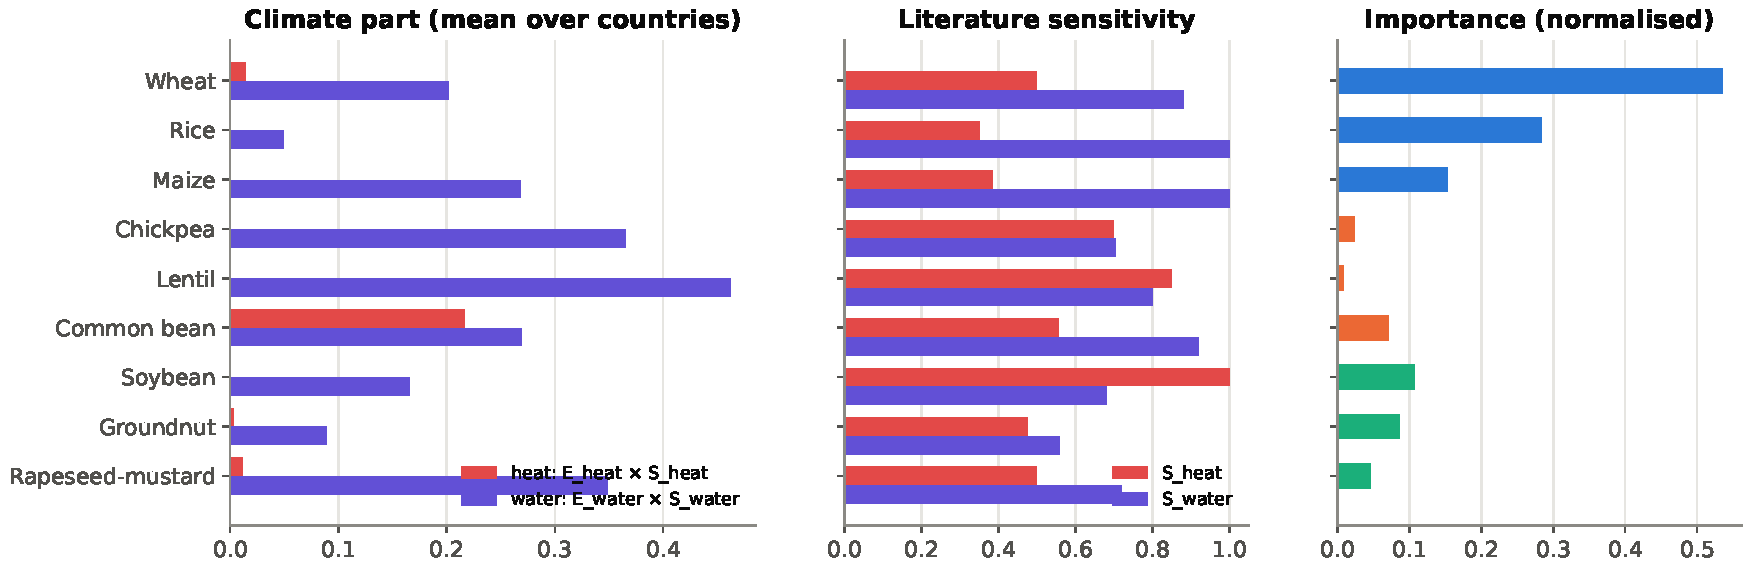
\includegraphics[width=\linewidth]{G03_components.pdf}\caption{Components by crop.}\end{figure}
\begin{figure}[H]\centering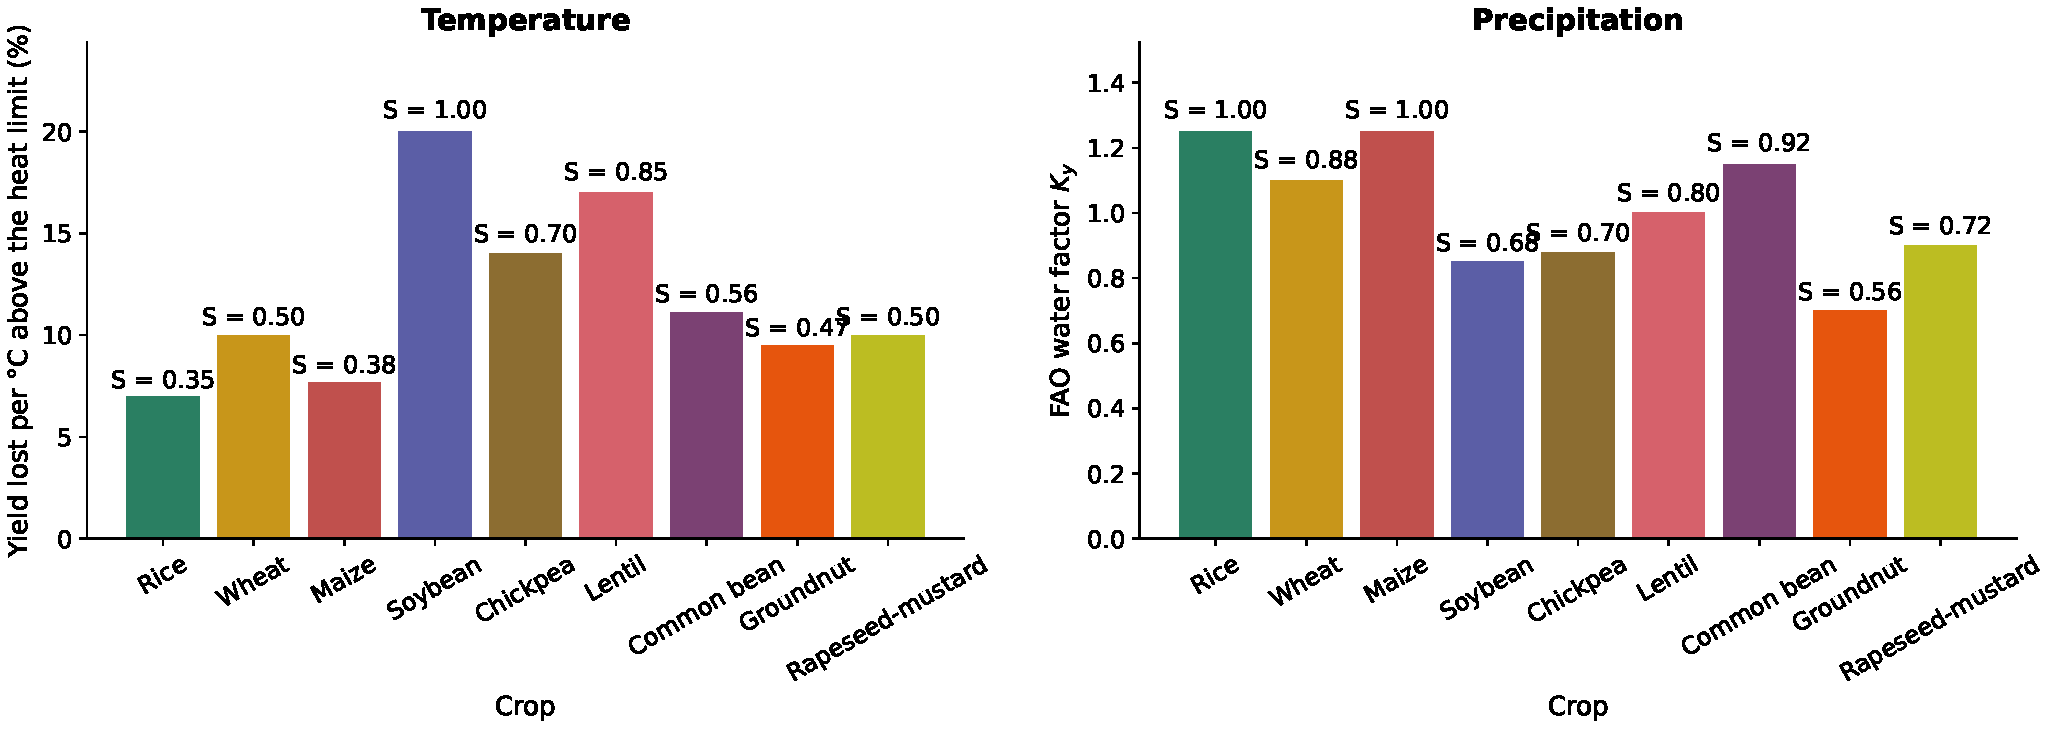
\includegraphics[width=0.9\linewidth]{F05l_literature_sensitivity.pdf}\caption{Literature sensitivity of the nine crops.}\end{figure}

\section{Future}
\begin{table}[H]\centering\small\caption{Crop scores 2001--24, 1971--2000 and 2041--2060.}
\adjustbox{max width=\linewidth}{\begin{tabular}{lrrrrrrcrrc}
\toprule
Crop & $\Delta T_{eff}$ & 2001--24 & 1971--2000 & 2041--60 & $\Delta$F4 & \% & rank eq & pairs up & F4 pw 2041--60 & rank pw \\
\midrule
Wheat & +2.0 & 0.0563 & 0.0535 & 0.0616 & +0.0080 & +15\% & 1$\to$1 & 6/6 & 0.0762 & 1$\to$1 \\
Maize & +2.0 & 0.0297 & 0.0263 & 0.0254 & -0.0009 & -3\% & 2$\to$2 & 3/6 & 0.0084 & 6$\to$6 \\
Common bean & +2.0 & 0.0172 & 0.0167 & 0.0224 & +0.0057 & +34\% & 3$\to$3 & 7/7 & 0.0276 & 3$\to$2 \\
Rapeseed-mustard & +2.0 & 0.0078 & 0.0076 & 0.0081 & +0.0006 & +8\% & 5$\to$4 & 7/7 & 0.0161 & 4$\to$4 \\
Soybean & +1.9 & 0.0078 & 0.0079 & 0.0080 & +0.0001 & +1\% & 4$\to$5 & 3/7 & 0.0121 & 5$\to$5 \\
Chickpea & +2.0 & 0.0053 & 0.0052 & 0.0053 & +0.0001 & +2\% & 6$\to$6 & 3/7 & 0.0227 & 2$\to$3 \\
Rice & +1.8 & 0.0024 & 0.0027 & 0.0022 & -0.0005 & -17\% & 7$\to$7 & 5/7 & 0.0016 & 9$\to$9 \\
Lentil & +2.2 & 0.0021 & 0.0021 & 0.0021 & -0.0000 & -1\% & 9$\to$8 & 4/7 & 0.0040 & 7$\to$7 \\
Groundnut & +1.6 & 0.0015 & 0.0021 & 0.0017 & -0.0004 & -19\% & 8$\to$9 & 2/5 & 0.0019 & 8$\to$8 \\
\bottomrule
\end{tabular}
\par\vspace{2pt}{\footnotesize MRI-ESM2-0, SSP2-4.5, change factors on 1971--2000 years; one fixed normalisation reference (2001--24 nine-crop maxima); sensitivity, importance, crop area, irrigation and calendars held fixed. $\Delta T_{eff}$ = mean change in flowering-window effective temperature (\si{\celsius}). \% only where the historical score is $\geq$1\% of the largest.}
}\end{table}
\begin{table}[H]\centering\small\caption{Largest pair increases.}
\adjustbox{max width=\linewidth}{\begin{minipage}{\textwidth}\centering
\adjustbox{max width=\textwidth}{\begin{tabular}{lrrrrrrr}
\toprule
Pair & 1971--2000 & 2041--60 & $\Delta$F4 & \% & from heat & from water & $\Delta T_{eff}$ \\
\midrule
Wheat--Russia & 0.1286 & 0.1493 & +0.0207 & +16\% & +0.0071 & +0.0136 & +2.5 \\
Common bean--Tanzania & 0.0385 & 0.0574 & +0.0188 & +49\% & +0.0094 & +0.0094 & +1.7 \\
Common bean--Brazil & 0.0409 & 0.0548 & +0.0139 & +34\% & +0.0112 & +0.0026 & +2.1 \\
Wheat--India & 0.0612 & 0.0717 & +0.0105 & +17\% & +0.0102 & +0.0003 & +1.5 \\
Wheat--USA & 0.0894 & 0.0998 & +0.0104 & +12\% & +0.0058 & +0.0046 & +2.4 \\
Maize--Ukraine & 0.0283 & 0.0327 & +0.0044 & +16\% & +0.0000 & +0.0044 & +3.3 \\
Soybean--USA & 0.0259 & 0.0297 & +0.0039 & +15\% & +0.0002 & +0.0037 & +3.1 \\
Wheat--Brazil & 0.0097 & 0.0124 & +0.0027 & +27\% & +0.0005 & +0.0021 & +1.7 \\
\bottomrule
\end{tabular}
}
\par\vspace{2pt}{\footnotesize Largest increases. 'from heat/water' = the change in each hazard term (future sensitivity and importance, fixed).}
\end{minipage}
}\end{table}
\begin{figure}[H]\centering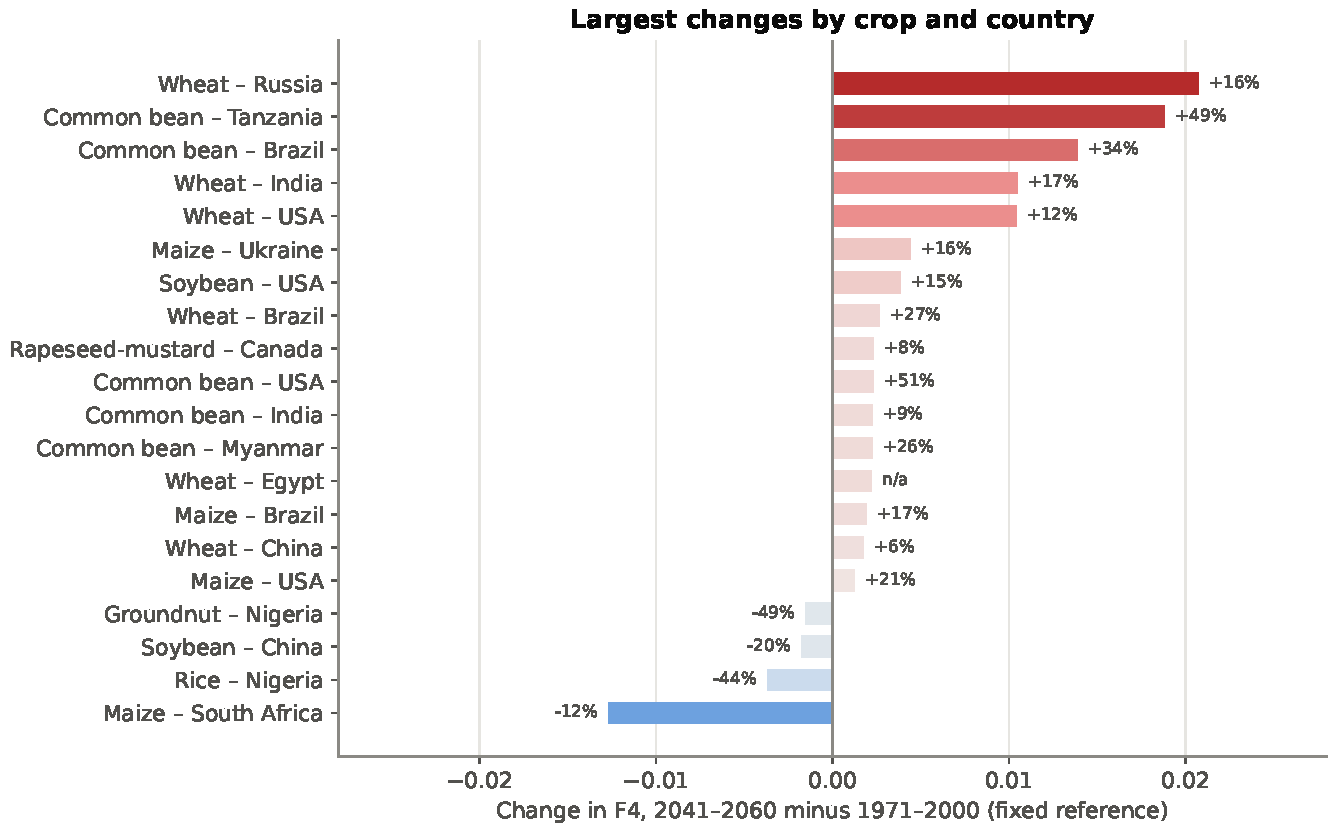
\includegraphics[width=0.8\linewidth]{G05_future_pairs.pdf}\caption{Largest changes by pair.}\end{figure}

\section{Nutrition}
\begin{table}[H]\centering\small\caption{Nutrient adequacy ratios, main and alternative requirements.}
\adjustbox{max width=\linewidth}{\begin{tabular}{lrrrrrrrrr}
\toprule
Country & kcal & protein & fat & Zn & Fe & MAR & Zn mod. & Fe 15\% & MAR alt \\
\midrule
Bangladesh & 1.00 & 1.00 & 1.00 & 1.00 & 0.70 & 93.9 & 1.00 & 1.00 & 100.0 \\
South Africa & 1.00 & 1.00 & 1.00 & 1.00 & 0.82 & 96.4 & 1.00 & 1.00 & 100.0 \\
Tanzania & 1.00 & 1.00 & 1.00 & 1.00 & 0.83 & 96.7 & 1.00 & 1.00 & 100.0 \\
Myanmar & 1.00 & 1.00 & 1.00 & 1.00 & 0.89 & 97.7 & 1.00 & 1.00 & 100.0 \\
India & 1.00 & 1.00 & 1.00 & 1.00 & 0.89 & 97.8 & 1.00 & 1.00 & 100.0 \\
Nigeria & 1.00 & 1.00 & 1.00 & 1.00 & 0.91 & 98.1 & 1.00 & 1.00 & 100.0 \\
Brazil & 1.00 & 1.00 & 1.00 & 1.00 & 0.97 & 99.4 & 1.00 & 1.00 & 100.0 \\
Australia & 1.00 & 1.00 & 1.00 & 1.00 & 1.00 & 100.0 & 1.00 & 1.00 & 100.0 \\
Egypt & 1.00 & 1.00 & 1.00 & 1.00 & 1.00 & 100.0 & 1.00 & 1.00 & 100.0 \\
China & 1.00 & 1.00 & 1.00 & 1.00 & 1.00 & 100.0 & 1.00 & 1.00 & 100.0 \\
Canada & 1.00 & 1.00 & 1.00 & 1.00 & 1.00 & 100.0 & 1.00 & 1.00 & 100.0 \\
Belarus & 1.00 & 1.00 & 1.00 & 1.00 & 1.00 & 100.0 & 1.00 & 1.00 & 100.0 \\
Italy & 1.00 & 1.00 & 1.00 & 1.00 & 1.00 & 100.0 & 1.00 & 1.00 & 100.0 \\
France & 1.00 & 1.00 & 1.00 & 1.00 & 1.00 & 100.0 & 1.00 & 1.00 & 100.0 \\
Ethiopia & 1.00 & 1.00 & 1.00 & 1.00 & 1.00 & 100.0 & 1.00 & 1.00 & 100.0 \\
Argentina & 1.00 & 1.00 & 1.00 & 1.00 & 1.00 & 100.0 & 1.00 & 1.00 & 100.0 \\
Russia & 1.00 & 1.00 & 1.00 & 1.00 & 1.00 & 100.0 & 1.00 & 1.00 & 100.0 \\
Turkey & 1.00 & 1.00 & 1.00 & 1.00 & 1.00 & 100.0 & 1.00 & 1.00 & 100.0 \\
Ukraine & 1.00 & 1.00 & 1.00 & 1.00 & 1.00 & 100.0 & 1.00 & 1.00 & 100.0 \\
USA & 1.00 & 1.00 & 1.00 & 1.00 & 1.00 & 100.0 & 1.00 & 1.00 & 100.0 \\
\bottomrule
\end{tabular}
\par\vspace{2pt}{\footnotesize NAR = min(1, national supply / requirement), 2021--23. Main: zinc low bioavailability, iron 10\% bioavailability (WHO/FAO 2004 RNIs). Alternative: moderate zinc, 15\% iron. RNIs are individual upper-percentile requirements compared with national mean supply, so both overstate shortfall.}
}\end{table}
\begin{table}[H]\centering\small\caption{Standard $-10\%$ shock.}
\adjustbox{max width=\linewidth}{\begin{minipage}{\textwidth}\centering
\adjustbox{max width=\textwidth}{\begin{tabular}{lrrrrrrrr}
\toprule
Pair & min(1,SSR) & $\Delta$kcal \% & $\Delta$prot \% & $\Delta$Zn \% & $\Delta$Fe \% & MAR & $\Delta$MAR & w/ exports \\
\midrule
Maize--South Africa & 1.00 & -2.17 & -2.20 & -2.95 & -3.23 & 96.4 & -0.53 & -0.00 \\
Wheat--India & 1.00 & -2.11 & -2.38 & -3.26 & -2.95 & 97.8 & -0.52 & -0.28 \\
Rice--Bangladesh & 1.00 & -6.29 & -4.74 & -5.45 & -3.62 & 93.9 & -0.50 & -0.50 \\
Common bean--Tanzania & 1.00 & -0.55 & -1.56 & -0.89 & -1.96 & 96.7 & -0.33 & -0.14 \\
Wheat--Brazil & 0.69 & -0.75 & -0.77 & -1.41 & -1.57 & 99.4 & -0.31 & +0.00 \\
Common bean--Brazil & 1.00 & -0.31 & -0.70 & -0.48 & -1.32 & 99.4 & -0.26 & -0.16 \\
Rice--India & 1.00 & -2.47 & -1.80 & -2.09 & -1.15 & 97.8 & -0.20 & -0.00 \\
Maize--Brazil & 1.00 & -0.72 & -0.50 & -0.92 & -1.05 & 99.4 & -0.20 & +0.00 \\
Groundnut--Nigeria & 0.99 & -0.55 & -0.71 & -0.56 & -0.52 & 98.1 & -0.09 & -0.09 \\
Common bean--India & 0.94 & -0.13 & -0.31 & -0.20 & -0.44 & 97.8 & -0.08 & -0.07 \\
Rice--Brazil & 1.00 & -0.78 & -0.52 & -0.59 & -0.40 & 99.4 & -0.08 & +0.00 \\
Chickpea--India & 1.00 & -0.23 & -0.51 & -0.34 & -0.40 & 97.8 & -0.07 & -0.06 \\
\bottomrule
\end{tabular}
}
\par\vspace{2pt}{\footnotesize Standard $-10\%$ yield shock, no market response; national supply 2021--23. MAR and $\Delta$MAR in points out of 100. 'w/ exports' = exports absorb the loss first.}
\end{minipage}
}\end{table}
\begin{table}[H]\centering\small\caption{Conditional future yield and nutrient change (largest MAR changes).}
\adjustbox{max width=\linewidth}{\begin{tabular}{lrrrrrr}
\toprule
Pair & $\Delta Y$ lit \% & $\Delta Y$ emp \% & $\Delta$kcal \% & $\Delta$Fe \% & $\Delta$MAR & w/ exports \\
\midrule
Common bean--Brazil & -25.6 & +0.0 & -0.80 & -3.39 & -0.66 & -0.57 \\
Common bean--Tanzania & -17.7 & +0.0 & -0.97 & -3.47 & -0.58 & -0.42 \\
Wheat--India & -4.2 & -6.5 & -0.88 & -1.23 & -0.22 & -0.00 \\
Common bean--India & -17.5 & +0.0 & -0.22 & -0.78 & -0.14 & -0.13 \\
Common bean--Myanmar & -21.5 & +0.0 & -0.19 & -0.74 & -0.13 & -0.00 \\
Maize--Brazil & -2.7 & -18.3 & -0.20 & -0.29 & -0.06 & +0.00 \\
Wheat--Brazil & -1.7 & -3.0 & -0.13 & -0.27 & -0.05 & +0.00 \\
Rice--Brazil & -0.8 & +0.0 & -0.06 & -0.03 & -0.01 & +0.00 \\
Groundnut--Brazil & -9.7 & -3.6 & -0.01 & -0.02 & -0.00 & +0.00 \\
Lentil--India & -2.0 & -0.6 & -0.01 & -0.02 & -0.00 & -0.00 \\
\bottomrule
\end{tabular}
\par\vspace{2pt}{\footnotesize Conditional screening estimate: change in climate-attributable loss (heat: $s_T \cdot$ \si{\celsius} above $T_{crit}$; water: $K_y \cdot$ rainfed deficit), 2041--60 vs 1971--2000, MRI-ESM2-0 SSP2-4.5; no CO$_2$ fertilisation, adaptation or market response. Only losses propagated.}
}\end{table}
\begin{figure}[H]\centering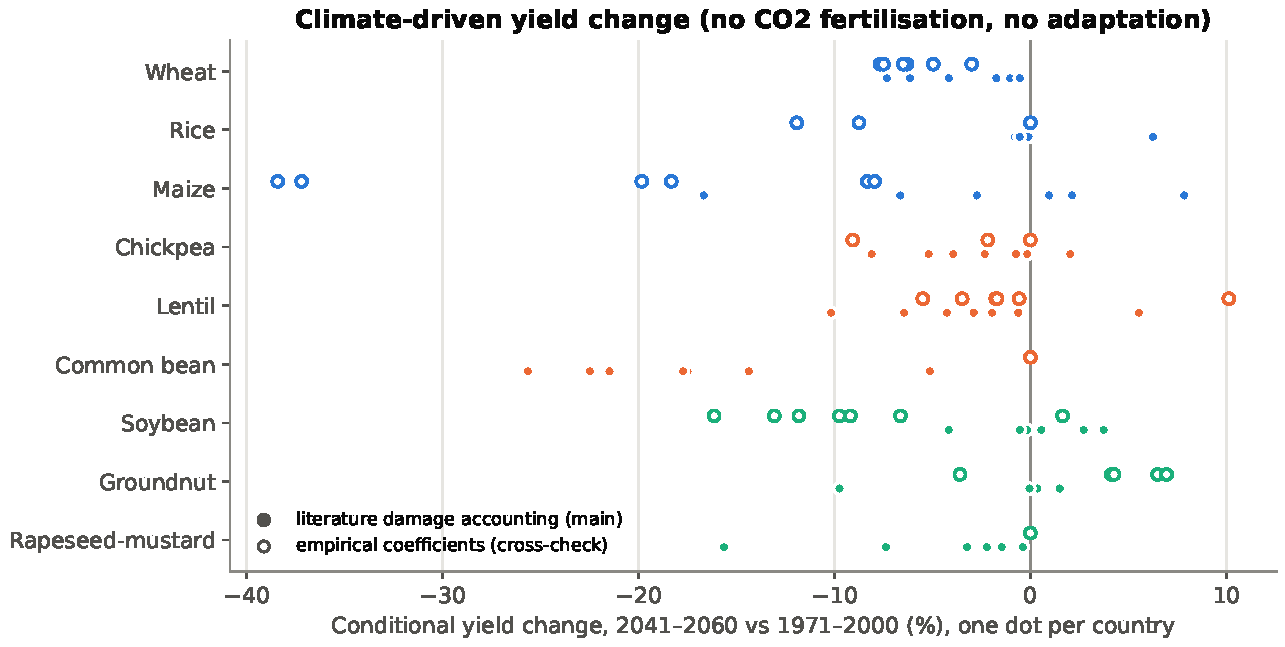
\includegraphics[width=0.9\linewidth]{G09_future_yield.pdf}\caption{Conditional yield change, literature vs empirical.}\end{figure}

\section{Robustness and validation}
\begin{table}[H]\centering\scriptsize\caption{One-at-a-time robustness tests.}
\adjustbox{max width=\linewidth}{\begin{tabular}{p{6.8cm}p{5.2cm}cc}
\toprule
Test (one at a time) & Top three, F4 equal weights & Wheat rank eq & rank pw \\
\midrule
main (x/max, exposure = stress level, literature S) & Wheat $>$ Maize $>$ Commo \ldots & 1 & 1 \\
min-max normalisation & Wheat $>$ Maize $>$ Commo \ldots & 1 & 1 \\
exposure = level + change (average) & Wheat $>$ Maize $>$ Rice \ldots & 1 & 1 \\
exposure = change only & Wheat $>$ Maize $>$ Rice \ldots & 1 & 1 \\
sensitivity = literature + empirical average (mid-evaluation configuration) & Wheat $>$ Maize $>$ Commo \ldots & 1 & 1 \\
sensitivity = empirical only & Soybe $>$ Lenti $>$ Wheat \ldots & 3 & 3 \\
rice Ky = 1.0 & Wheat $>$ Maize $>$ Commo \ldots & 1 & 1 \\
rice Ky = 1.5 & Wheat $>$ Maize $>$ Commo \ldots & 1 & 1 \\
importance = kcal share only & Wheat $>$ Maize $>$ Soybe \ldots & 1 & 1 \\
importance = Zn+Fe+protein only & Wheat $>$ Maize $>$ Commo \ldots & 1 & 1 \\
heat threshold T crit -2 C (all crops) & Wheat $>$ Maize $>$ Commo \ldots & 1 & 1 \\
heat threshold T crit -1 C (all crops) & Wheat $>$ Maize $>$ Commo \ldots & 1 & 1 \\
heat threshold T crit +1 C (all crops) & Wheat $>$ Maize $>$ Commo \ldots & 1 & 1 \\
heat threshold T crit +2 C (all crops) & Wheat $>$ Maize $>$ Commo \ldots & 1 & 1 \\
heat threshold T crit +3 C (all crops) & Wheat $>$ Maize $>$ Commo \ldots & 1 & 1 \\
new legumes T crit +3 C (chamber vs model thresholds) & Wheat $>$ Maize $>$ Commo \ldots & 1 & 1 \\
bean T crit +2 C (Mesoamerican types) & Wheat $>$ Maize $>$ Commo \ldots & 1 & 1 \\
calendar = plain Sacks (Pulses / Rapeseed.Winter) for chickpea, lentil, rapeseed & Wheat $>$ Maize $>$ Commo \ldots & 1 & 1 \\
new legumes: heat slope x0.7 (chamber -> field) & Wheat $>$ Maize $>$ Commo \ldots & 1 & 1 \\
rapeseed heat slope 0.07 (proxy low) & Wheat $>$ Maize $>$ Commo \ldots & 1 & 1 \\
rapeseed heat slope 0.18 (proxy high) & Wheat $>$ Maize $>$ Commo \ldots & 1 & 1 \\
new crops K y low (chickpea 0.67, lentil 0.87, bean 0.6, rapeseed 0.85) & Wheat $>$ Maize $>$ Commo \ldots & 1 & 1 \\
new crops K y high (chickpea 1.15, lentil 1.15, bean 1.4, rapeseed 0.95) & Wheat $>$ Maize $>$ Commo \ldots & 1 & 1 \\
\bottomrule
\end{tabular}
}\end{table}
\begin{figure}[H]\centering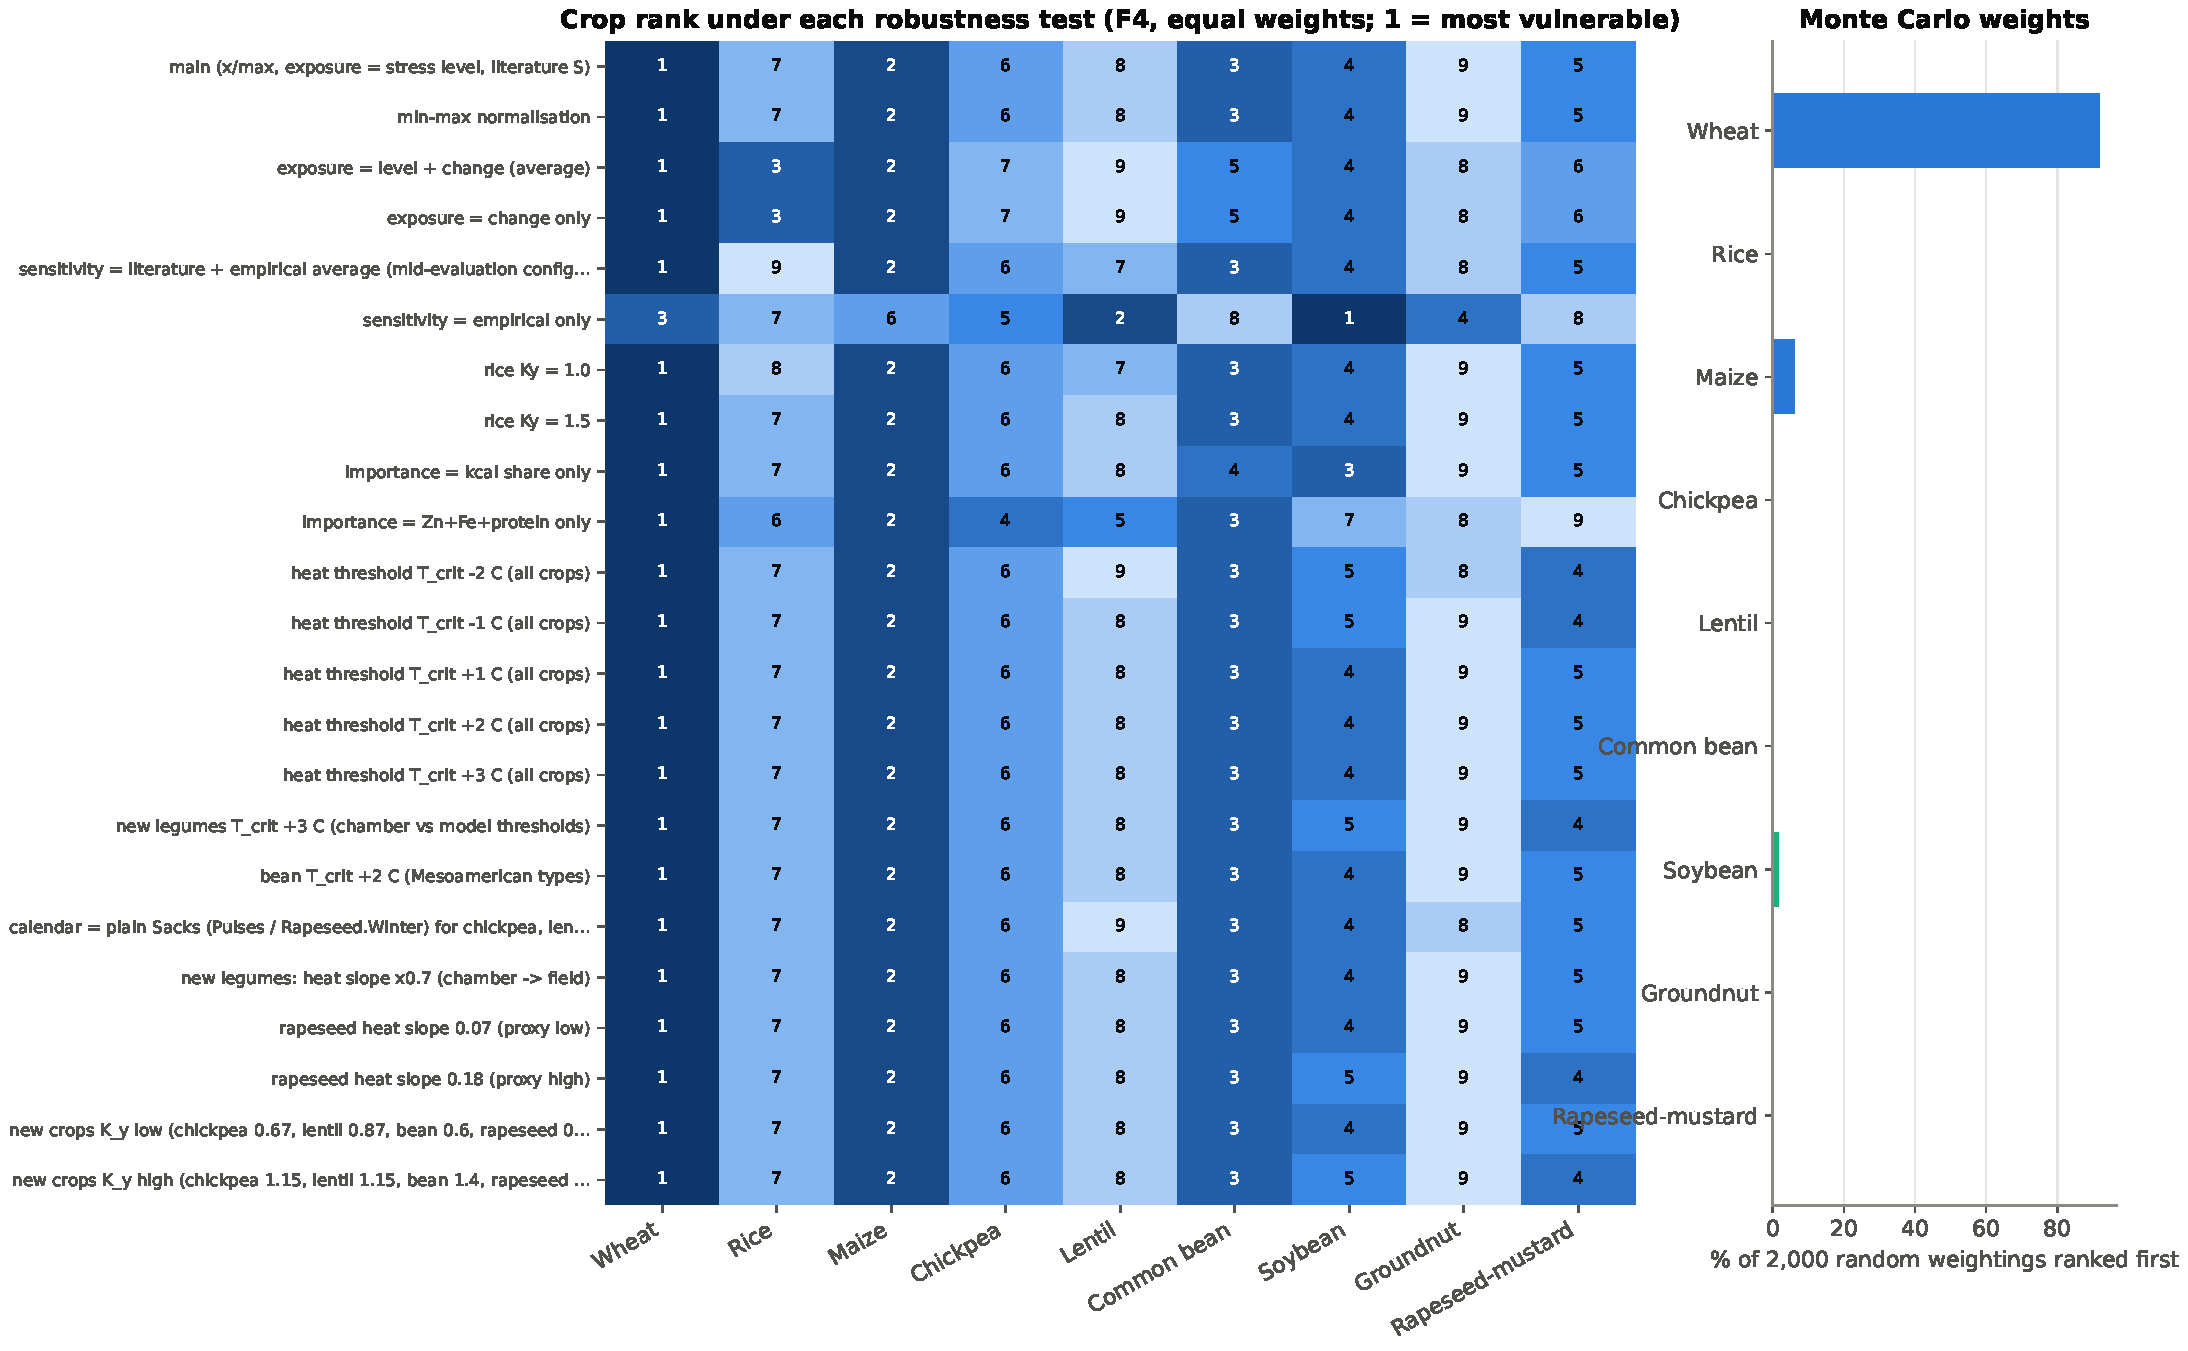
\includegraphics[width=\linewidth]{G10_robustness.pdf}\caption{Ranks under each test and Monte Carlo.}\end{figure}
\begin{table}[H]\centering\scriptsize\caption{Comparison with published findings.}
\begin{minipage}{\textwidth}\centering
\adjustbox{max width=\textwidth}{\begin{tabular}{p{0.9cm}p{3.0cm}p{4.4cm}p{4.6cm}p{2.0cm}}
\toprule
 & Study & Published finding & Our comparable result & Verdict \\
\midrule
Z1 & Zhao et al. 2017 PNAS & yield change per +1 C: maize -7.4, wheat -6.0, rice -3.2, soybean -3.1 (n.s.) -$>$ maize $>$ wheat $>$ rice $>$ soybean & climate part E x S (equal weights): maize $>$ wheat $>$ soybean $>$ rice; Spearman rho with Zhao = +0.8 (n = 4) & agree (order of maize, wheat) \\
Z2 & Zhao et al. 2017 PNAS (Fig. 3) & wheat loss per +1 C: India -9.1, Russia -7.8, USA -5.5, China -2.6 \% & wheat heat exposure E\_heat: India 0.115, Russia 0.015, USA 0.015, China 0.002 & agree (heat) \\
L1 & Lobell, Schlenker \& Costa-Roberts 2011 Science & Russia wheat production about -15 \% from temperature trends & wheat-Russia F4 = 0.1315 (top pair); heat part 0.0027 vs water part 0.1288 & differ (mechanism) \\
R1 & Ray et al. 2015 Nat. Commun.; Ray et al. 2019 PLoS ONE & climate explains 32-39 \% of yield variability; rice least & rice climate part E x S = 0.0247, lowest of the four (wheat 0.1077, maize 0.1345, soybean 0.0830) & not directly comparable (different outcome) \\
D1 & Deryng et al. 2014 ERL (Table 1) & maize -10.5, wheat -10.1, soybean -6.9 \% (RCP4.5 with CO2: -4.9, +13.0, +10.8) & our conditional yield change (mean over countries, no CO2): maize -2.5 \%, wheat -3.5 \%, soybean +0.7 \% & sign agrees for maize; sign agrees for wheat; sign differs for soybean; our magnitudes smaller \\
C1 & Challinor et al. 2014 Nat. Clim. Change & $>$ 70 \% of projections show yield losses & 76 \% of our 59 pairs show a climate-driven yield loss (literature accounting); cereals only: 74 \% & agree \\
RC & Ramirez-Cabral et al. 2017 Sci. Rep. & suitable area: Africa -7 to -11 \%, South America -5 \%, India marginal areas become unsuitable & maize change in F4 2041-60 vs 1971-2000: South Africa -0.0127, Brazil +0.0019, India -0.0002 & differ \\
RP/HU & Rippke et al. 2016 Nat. Clim. Change; Hummel et al. 2018 Sci. Rep. & beans -10 \% area needing transformation in Uganda/Tanzania by the 2050s (RP); most SE African bean areas unsuitable by 2040-69, drought-driven (HU) & bean-Tanzania F4 change +0.0188; conditional yield change -17.7 \% & agree (direction) \\
Q1 & Qian et al. 2019 ERL (Table 2) & -0.8 to -5.7 \% production at +2 C with CO2 fixed (+3 to +11 \% with CO2) & rapeseed-Canada conditional yield change -3.2 \% (no CO2); flowering T\_eff change +3.1 C & agree (sign) \\
K1 & Kalra et al. 2008 Curr. Sci. & yields fall with warmer seasons: chickpea -0.53 to -3.01, mustard -0.92 to -2.01 q/ha per C & India 2041-60: chickpea T\_eff +1.3 C, yield -0.2 \%; rapeseed-mustard T\_eff +1.6 C, yield -2.2 \% & agree (sign) \\
BE/NE & Beach et al. 2019 Lancet Planet. Health; Nelson et al. 2018 Nat. Sustain. & South Asia iron availability below the recommended intake; micronutrients, not calories, are the binding constraint & India 2021-23 iron supply / requirement = 0.89 (15 \% bioavailability: 1.00); energy 1.00, protein 1.00 & agree (main requirement) \\
M1 & Myers et al. 2014 Nature & iron concentration: wheat -5.1, rice -5.2, soybean -4.1 \% (significant) & applied to India's 2021-23 iron supply shares, these declines alone would lower national iron supply by 2.2 \% (an additional pathway the index excludes) & additional pathway \\
\bottomrule
\end{tabular}
}
\par\vspace{2pt}{\footnotesize Signs and rank orders only; published values verified in docs/literature\_comparison\_sources.md; ours computed by code/22\_literature\_comparison.py.}
\end{minipage}
\end{table}

\section{Mid-evaluation record and the presented method}
The mid-evaluation numbers used blended sensitivity; the four-crop run with the presented literature-only
method gives the same crop order (\orderFourEq; production-weighted \orderFourPw) with higher values
(median ratio \litRatioMedian) and a new top pair, \litTopPair\ (\litTopValue) just ahead of \litSecondPair\
(\litSecondValue). The regenerated four-crop figure and table set is in \texttt{figures/four\_crop/} and
\texttt{docs/four\_crop/generated/}; the frozen mid-evaluation record is in \texttt{archive/mid\_evaluation/}.
\begin{figure}[H]\centering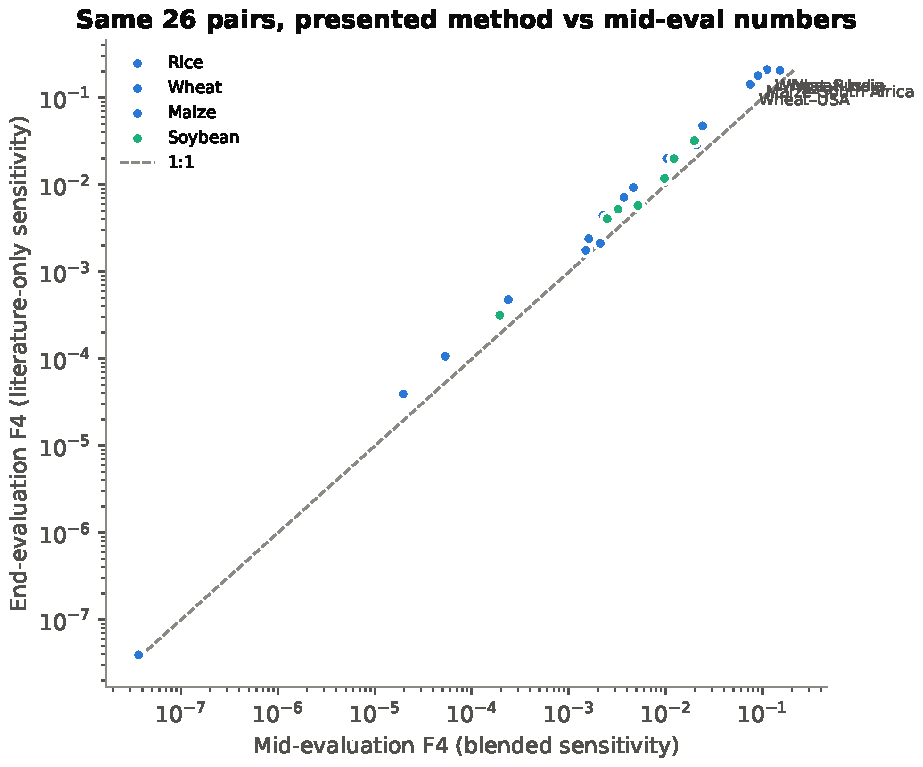
\includegraphics[width=0.6\linewidth]{G11_mideval_vs_literature_only.pdf}\caption{Same 26 pairs: mid-evaluation vs presented method.}\end{figure}

\bibliography{refs}
\end{document}
